\documentclass{article}
\usepackage{tikz}
\usepackage{tkz-euclide}
\usetikzlibrary{calc,intersections}
\usepackage{graphicx}
\newcommand{\Wheel}[3]{
  \begin{scope}[shift={#1},rotate=#2]
    \draw[rounded corners=9,#3] (-1,-5) rectangle (1,5);
  \end{scope}
}

\begin{document}

\bigskip
\begin{tikzpicture}[x=3mm,y=3mm]
  \draw (0,0) -- (10,0);
  \draw[fill,red] (-0.3,0) rectangle (0.3,20);
  \Wheel{(0,0)}{0}{black};
  \begin{scope}[shift={(0,20)},rotate=40]
    \draw[dashed] (0,-7) -- (0,7);
    \draw[dashed] (3,0) -- (-35,0);
    \Wheel{(0,0)}{0}{black};
  \end{scope}
  \coordinate (P) at (-{20/tan(40)},0);
  \draw[red] (P) circle [radius=2pt];
  \draw[dashed] (0,0) -- (P);
  % \Wheel{(0,20)}{60}{red!30!blue};
\end{tikzpicture}


\section*{Geometric Path Planning}

Using Mozzi-Chasles' theorem, any rigid body displacement can be produced by a combination of
translation along a line and a rotation about an axis parallel to that line.

Given the initial location and heading at both the starting point and target points,
we want to compute the path comprised by translation and rotation as described by 
the above theorem.
We will analyze two different cases depending on the relative orientation between the heading
at the starting point and the heading at the target point.

\begin{itemize}
  \item When the relative orientation is larger than 90 degrees, the path requires
  only a single turn
  \item When the relative orientation is smaller than 90 degrees, the path can be solved
  using a single turn. However, there is a shorter path that includes two turns
\end{itemize}
\subsection*{A Single Turn}
\begin{figure}[hbt]  
  \begin{tabular}{cc}
    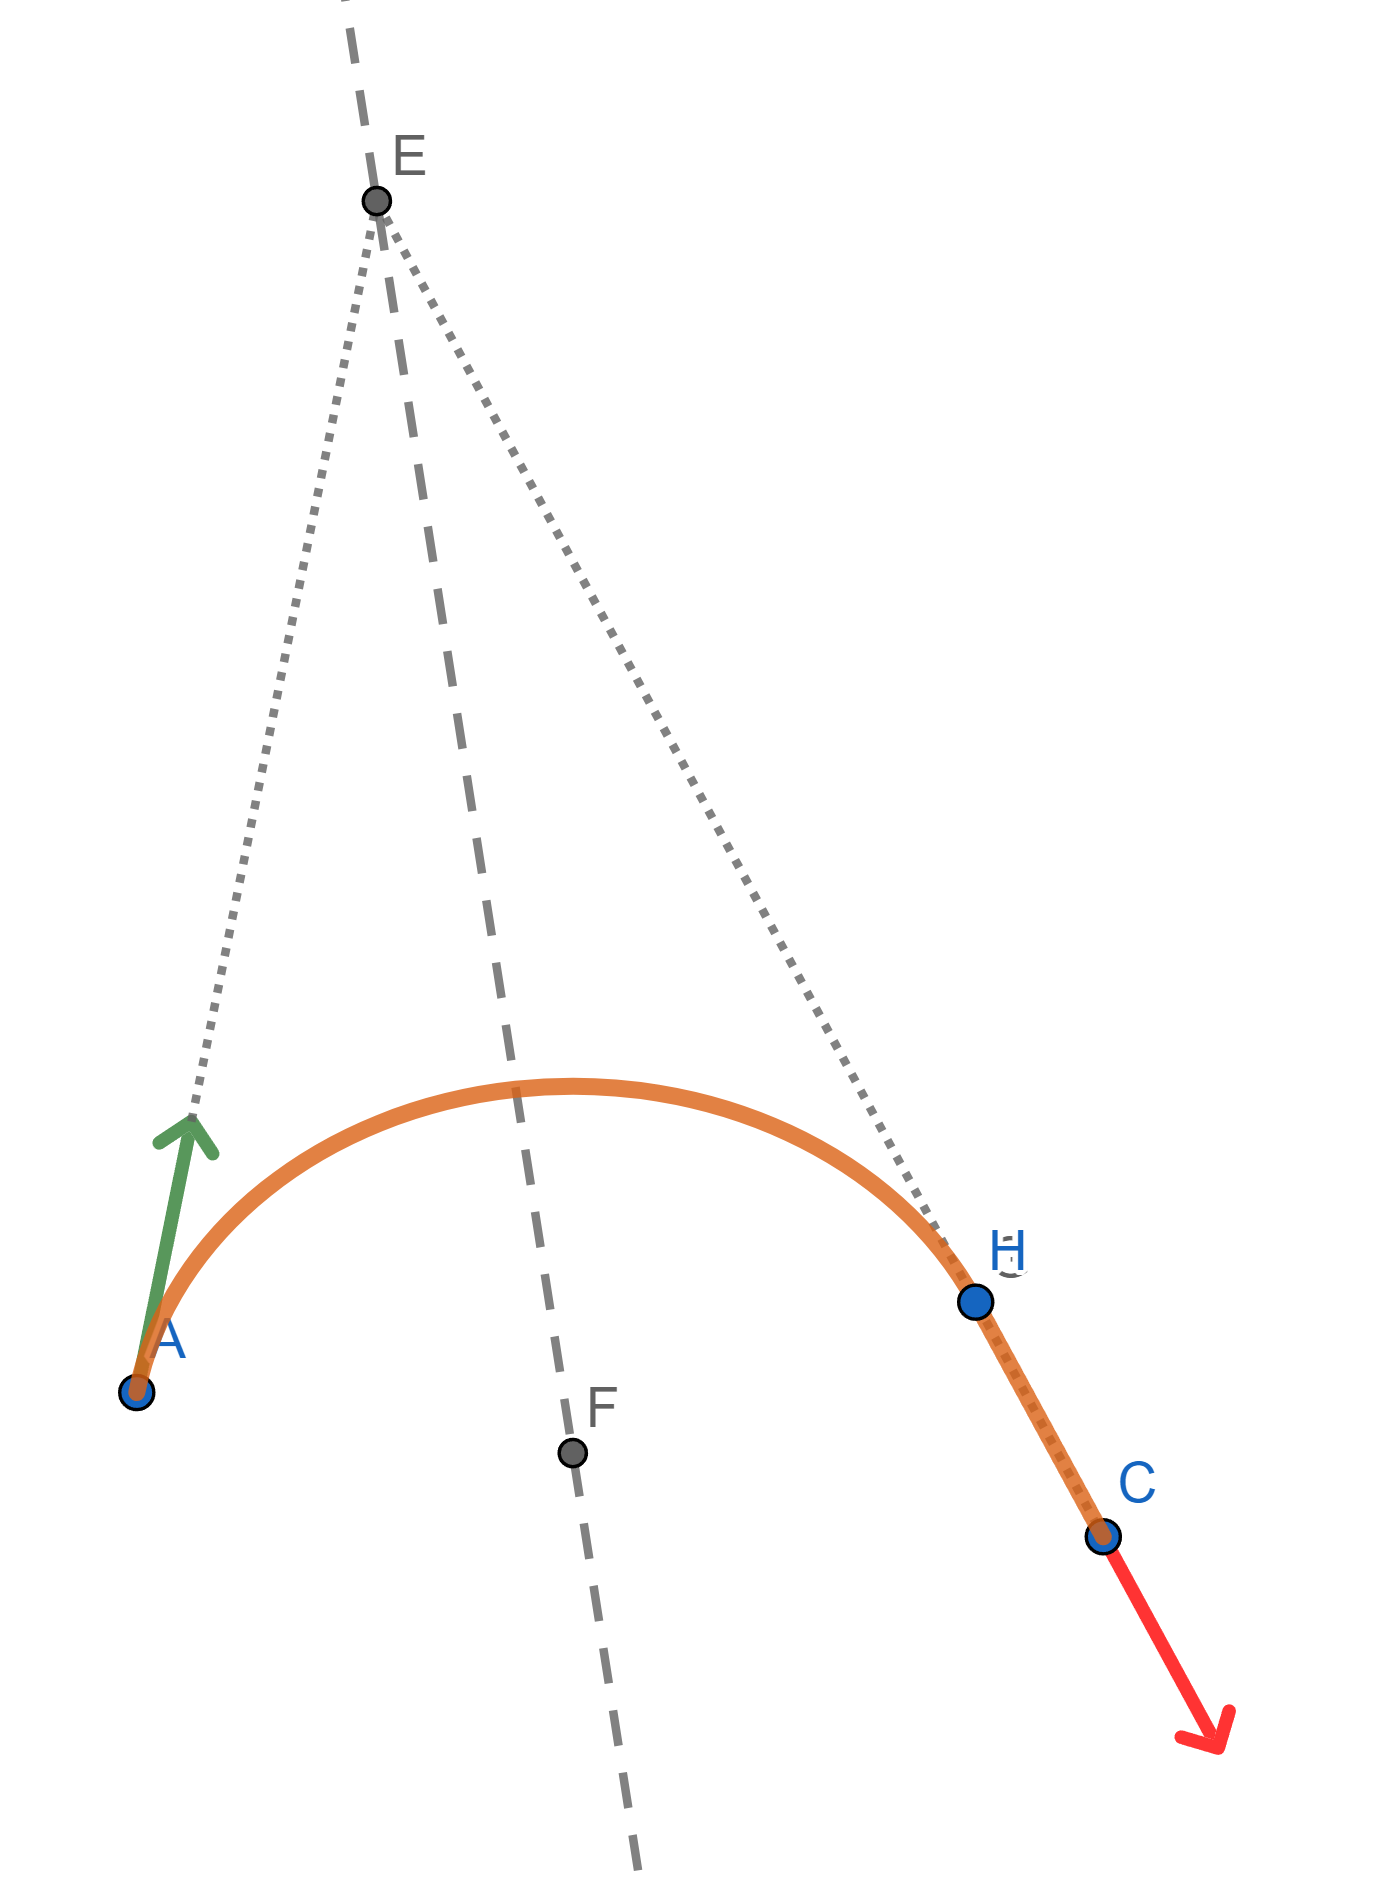
\includegraphics[width=3in]{screenshots/single-acute-turn-rot-trans.png} &
    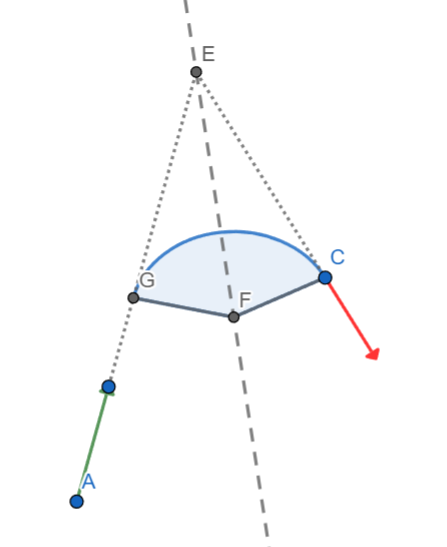
\includegraphics[width=3in]{screenshots/single-acute-turn-trans-rot.png}\\
    (a) & (b)\\
  \end{tabular} 
  \caption{Path planning with a single acute turn}
  \label{fig:path1turnacute}
\end{figure}


\begin{figure}[hbt]  
  \begin{tabular}{cc}
    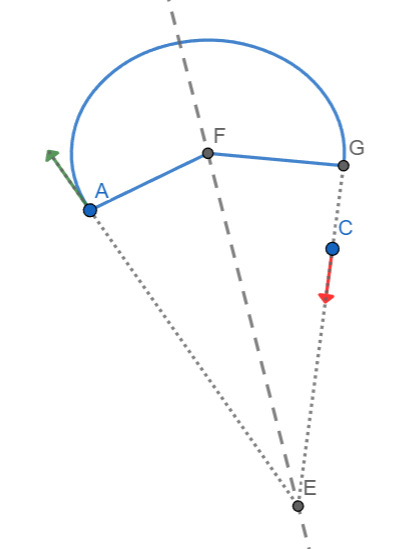
\includegraphics[width=3in]{screenshots/single-obtuse-turn-rot-trans.png} &
    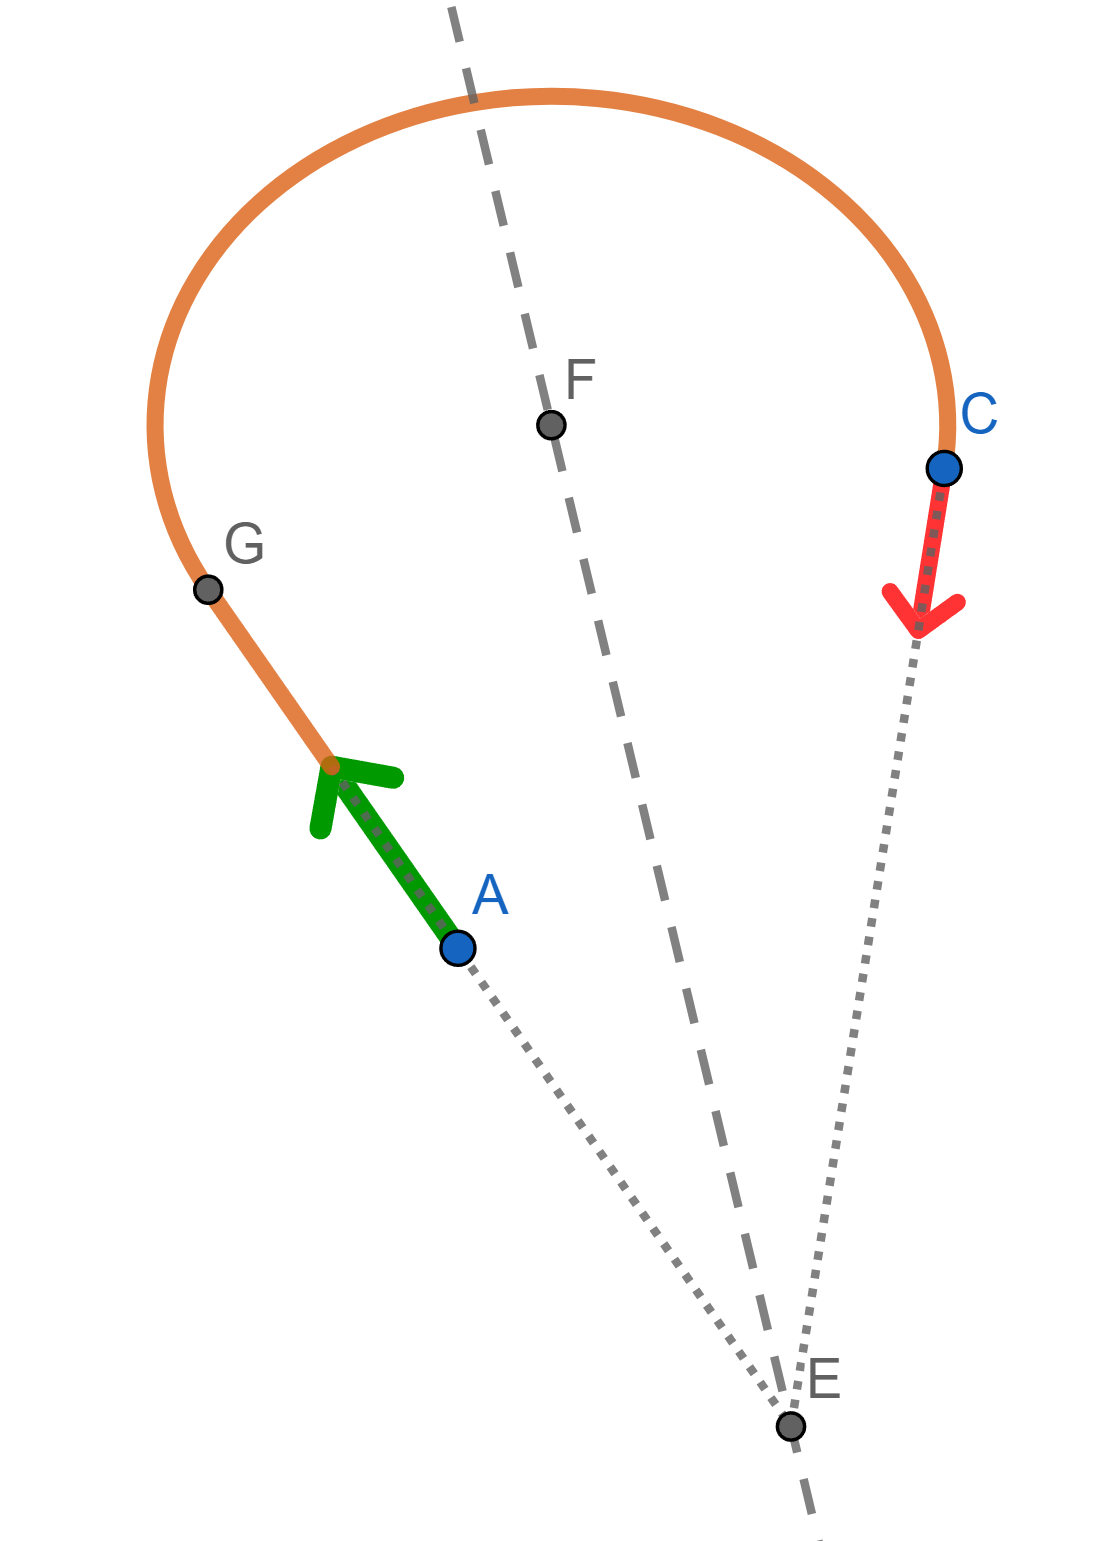
\includegraphics[width=3in]{screenshots/single-obtuse-turn-trans-rot.png}\\
    (a) & (b)\\
  \end{tabular} 
  \caption{Path planning with a single obtuse turn}
  \label{fig:path1turnobtuse}
\end{figure}

In Figure~\ref{fig:path1turnacute}, the bike starts at point $A$ with its heading shown by
the green arrow and its target is point $C$ with its heading shown by the red arrow.
The extending headings are shows by the dotted lines intersected at $E$.
Line $EF$ is the angle bisector of the both heading lines, and point $F$ is the
pivot of rotation.

There are two cases to consider:
\begin{itemize}
  \item In Figure~\ref{fig:path1turnacute}a, when $|AE| < |CE|$, the bike first rotates from $A$ and $G$ around the 
  pivot $F$  before it continues to translate from $G$ to $C$. In this case the pivot of rotation $F$ is determined
  by the starting point $A$
  \item In Figure~\ref{fig:path1turnacute}b, when $|AE| > |CE|$, the bike first translates from $A$ to $G$ before it 
  continues to rotate from $G$ to $C$ around the pivot $F$. In this case the pivot of rotation $F$ is determined
  by the target point $C$.
\end{itemize}
Notice that when the turn angle is acute, the pivot of rotation is determined by the \textbf{closer} 
of the starting/target point to the intersection $E$.
However, when the turn angle is obtuse, the pivot or rotation is determined by the \textbf{further}
point (as shown in Figure~\ref{fig:path1turnobtuse}).

\end{document}